% !TEX encoding = UTF-8 Unicode

\documentclass[a4paper]{article}

\usepackage{color}
\usepackage{url}
\usepackage[T2A]{fontenc} % enable Cyrillic fonts
\usepackage[utf8]{inputenc} % make weird characters work
\usepackage{graphicx}

\usepackage[english,serbian]{babel}
%\usepackage[english,serbianc]{babel} %ukljuciti babel sa ovim opcijama, umesto gornjim, ukoliko se koristi cirilica

\usepackage[unicode]{hyperref}
\hypersetup{colorlinks,citecolor=green,filecolor=green,linkcolor=blue,urlcolor=blue}

%\newtheorem{primer}{Пример}[section] %ćirilični primer
\newtheorem{primer}{Primer}[section]
\usepackage{graphicx}

\begin{document}

\title{Sinteza bioloških modela iz mutacijskih eksperimenata\\ \small{Seminarski rad u okviru kursa\\Verifikacija softvera\\ Matematički fakultet}}

\author{Una Stanković\\una\_stankovic@yahoo.com}
\date{26.~april 2018.}
\maketitle

\abstract{U ovom radu biće izneta osnovna ideja rada pod nazivom "Sinteza bioloških modela iz mutacijskih eksperimenata" (engl. Synthesis of Biological Models from Mutation Experiments) \cite{paper}. }

\newpage

\section{Uvod}
\label{sec:uvod}
Računarsko modelovanje bioloških sistema postaje sve popularnije sa pokušajima naučnika da u potpunosti razumeju kompleksne biološke fenomene.
Razlikuju se dva tipa bioloških problema, u zavisnosti od njihove reprezentacije i potencijala:
\begin{itemize}
\item matematički i
\item računarski
\end{itemize} 
Pristup, u kome od biloških sistema konstruišemo računarske modele, nazivamo "izvršivom biologijom" pošto se ona fokusira na dizajn algoritama, koji imitiraju biološke fenomene, a mogu da se izvršavaju na računaru.\cite{execbio} \\\\
Izvršiva biologija predstavlja novi izazov formalnim metodama.
Naime, javljaju se dva problema sa kojima se susreću biolozi koji se bave ćelijama kada razvijaju modele koji mogu da se analiziraju formalno.\\ Prvi se odnosi na automatsko sintetizovanje konkurentnog $"$in silico$"$ modela (onog koji se izvršava na računaru) za razvoj ćelija sa datim $"$in vivo$"$ eksperimentima (onima koji koriste žive jedinke) u kojima se ispituje kako određene mutacije utiču na ishod eksperimenta. Problem leži u tome što je sinteza, koja se vrši pod mutacijama, jedinstvena, jer mutacije mogu proizvesti nedeterminističke ishode i sintetizovani model mora biti u stanju da ponovi sve te ishode sa ciljem da verno opiše modelovane ćelijske procese. Suprotno tome, običan konkurentni program je korektan ako bira bilo koji ishod koji je predviđen nedeterminističkom specifikacijom. \\
Drugi se odnosi na problem nedovoljno ograničene specifikacije koji se javlja zbog nepotpunosti setova mutacijskih eksperimenata. Nedovoljno ograničena specifikacija prouzrokuje veći broj različitih modela, koji na različite načine objašnjavaju iste fenomene. Problem ovakve specifikacije odgovara problemu analize prostora zadovoljivih modela. U radu su razvijeni algoritmi koji otkrivaju dvosmislenosti u specifikaciji i uklanjaju redundantnost iz specifikacije, odnosno, kreiraju minimalnu nedvosmislenu specifikaciju.

\subsection{Motivacija}
Bolesti mogu biti uzrokovane izmenama na genu ili mrežama za regulaciju proteina. Uzmimo za primer bolest X koja je usko povezana sa nivoima nekih proteina, na primer, P i R, gde P može negativno regulisati nivo proteina R. Ako bi se desilo da nivo proteina P opadne, došlo bi do povećanja nivoa proteina R što bi mogao biti okidač za bolest X. Da bi se to izbeglo trebalo bi povećati nivo proteina R. Da bi bilo moguće izmeniti mreže regulacije proteina trebalo bi izvesti mutacioni eksperiment, u kome bi ćelije bile genetski modifikovane kako bi se smanjila ili povećala aktivnost određenog proteina. Kao posledica toga ćelija ispoljava abnormalno ponašanje, kao na primer nekontrolisanu deobu. Ako bi, umanjenjem aktivnosti proteina P, rezultujući fenotip ispoljio povećanu aktivnost proteina R, onda bi bilo moguće zaključiti da P negativno reguliše R. Iz ogromnog broja ovakvih eksperimenata biolozi dolaze do zaključaka i kreiraju regulatorne mreže koje opisuju posledice događaja koji dovode do određenih ćelijskih ponašanja i sudbina. Najpoznatiji primer kod kojih izmene dovode do bolesti je rak. Rak predstavlja grešku u regulaciji rasta tkiva kod kog su ćelije ispoljile izmenjeno ponašanje, odnosno, došlo je do izmene na genima koji regulišu rast ćelija.\\\\

Upravo kao posledica svega navedenog, eksperimentalnim biolozima je bitna korektnost modela koje kreiraju kao i detaljno objašenjenje kako je došlo do određenih ishoda. Izvršiva biologija se upravo bavi ovakvim problemima, kreiranjem izvršivih modela koji bi bili proverivi nad izvršenim eksperimentima. Tretiranje ćelija kao konkurentnih agenata modeluje činjenicu da ćelije ne evoluiraju istovremeno. Verifikacija obezbeđuje da je konkurentni model korektan za sve varijacije rasta ćelija, ispitivanjem svih mogućih izvršavanja modela.
Jedan od glavnih ciljeva eksperimentalne biologije je da stvori izvršive modele koji bi omogućili posmatranje dinamičnih bioloških sistema, koji bi bili potvrđeni kroz eksperimente. Da bi se transformisao neformalni model u izvršni moraju se modelovati:
\begin{itemize}
\item nivoi proteina,
\item vreme u kom proteini reaguju sa drugim komponentama i
\item ponašanje proteina kada su aktivni i aktivatorski i inhibitorski protein.
\end{itemize}

Mutacioni eksperimenti proizvode različite ishode kada se izvršavaju više puta. Korektan model bi morao da reprodukuje sve nedetrminističke ishode eksperimenta. Korišćenjem vezane asinhronizacije postiže se efekat da sve susedne ćelije uvek napreduju na sličan način, ali ne u potpunosti istovremeno. 

\section{Jezik}
\subsection{Jezik za modelovanje}
Jezik koji služi za modelovanje opisanih fenomena je model visokog nivoa, SBL, koji uvodi abstrakcije ćelija, ćelijskih komponenti i interakcija između njih. \\
Programi u SBL-u se sastoje iz ćelija, koje se izvršavaju prema određenom rasporedu $s$ koji koristi vezanu asinhronizaciju. Ćelije se sastoje iz komponenti, koje modeluju ili proteine ili receptore ćelija. Komponente jedne ćelije su u potpunosti sinhronizovane, međusobno komuniciraju na nivou jedne ili više ćelija i povezane su usmerenim granama, koje odgovaraju aktivacionim ili inhibitorskim vezama. Osim navedenog, komponente imaju stanje, koje se menja na osnovu stanja te komponente i stanja njenih aktivatora i inhibitora. Svaka komponenta ima, dakle, i funkciju promene stanja $(L, L^k) \longrightarrow L$, gde su $L$ nivoi, a $k$ broj aktivatora i inhibitora komponenti. 

\subsection{Dodaci jeziku za verifikaciju}
Skup mutacionih eksperimenata koji su izvedeni u laboratoriji služe za proveru korektnosti specifikacije. Sada, treba definisati određene pojmove:
\begin{itemize}
\item $F$ je skup mogućih ishoda eksperimenta.
\item $M$ je skup mutacija koje je moguće primeniti na ćeliju (obično su sve ćelije u eksperimentu isto mutirane). Ovaj skup raste eksponencijalno sa brojem komponenti ćelije, zbog čega biolozi ne izvode sve mutacije.
\item $Exp$ je skup eksperimenata, koji predstavlja podskup od $M \times F$, gde $(m,f) \in Exp$ ako je neki ishod $f$ uočen na mutaciji $m$. Pošto je skup eksperimenata nepotpun i specifikacija je nepotpuna. Zbog toga, pretpostavka, da kada je jednom izvršena mutacija laboratorija je proverila sve moguće ishode ponavljajući eksperiment dovoljan broj puta, nam omogućava da imamo gornju granicu za specifikaciju i da sintetizujemo i pozitivne(oni ishodi koje model mora proizvesti) i negativne primere(oni ishodi koji se nikad ne smeju uzeti za eksperiment).
\item Specifikacija je mapa $E: M \longrightarrow 2^F$, čiji je domen skup izvedenih mutacija. Ako je $m \in dom(E) \and f \notin E(m)$ pretpostavljamo da $m$ neće imati sudbinu $f$, tj. par $(m,f)$ je negativan primer.
\item Program $P: M \longrightarrow F$ je korektan model za $E$ ako se za svako $m \in dom(E)$ izvršavanjem programa $P$ dobija svaki element iz $E(m)$ kontrolisanjem rasporeda koji utiče na konkurentno izvršavanje ćelija u programu.
\end{itemize}
Da bi se definisao uslov korektnosti, program se mora posmatrati kao funkcija $P: (M,S) \rightarrow F$, gde su $M$ i $F$ domeni mutacija i sudbina ćelija,a $S$ predstavlja skup rasporeda koji koristi vezanu asinhronizaciju. Uslov korektnosti $correct(P,E)$ programa $P$ za specifikaciju $E: M \rightarrow 2^F$ ima dva dela:
\begin{enumerate}
\item demonsko raspoređivaje - ovakav vid rasporeda ne može proizvesti ishod koji je van specifikacije,
\item anđeosko raspoređivanje - ovakav vid rasporeda mora proizvesti svaki ishod iz specifikacije.
\end{enumerate}
\subsection{Dodaci jeziku za sintezu}
Jezik dozvoljava parametrizaciju ponašanja ćelijskih komponenti i načina njihove komunikacije. Korektan model mora reprodukovati sve uočene eksperimente, što je obuhvaćeno anđeoskim uslovom korektnosti, koji predstavlja formulu sa dva nivoa kvantifikacije(2NK). Iz toga sledi da je problem sinteze formula sa tri nivoa kvantifikacije(3NK). Formule koje su višeg nivoa kvantifikacije od 1 ne mogu se dati direktno SMT rešavaču na analizu. Kao posledica navedenog, autori su razvili dvokoračni CEGIS (engl. counterexample-guided inductive synthesis) algoritam, u kom sintetizer komunicira sa dva proverivača korektnosti (za anđeoski i demonski uslov).

\section{Sinteza i ispitivanje prostora modela}
Uslov korektnosti je definisan kao 
\begin{equation}
correct(P) = demonic(P) \land angelic(P)
\end{equation}
Korektnost utvrđujemo odvojeno za $demonic(P)$ i $angelic(P)$ pomoću verifikatora $V_d$ i $V_a$.\\
Kod demonskih rasporeda formula $demonic(P)$ tvrdi da je skup $E(m)$ gornja granica za sve ishode $P$ sa ulazom $m$:
\begin{equation}
demonic(P) = \forall m \in dom(E). \forall s \in S. P(m,s) \in E(m)
\end{equation}
Da bi se ovaj uslov proverio, mora se oboriti traženjem demonskog rasporeda takvog da, za neki ulaz iz $dom(E)$, proizvodi nepredviđeni ishod. S obzirom na to da je mali skup ulaznih vrednosti u $dom(E)$ formulu rešavamo tako što simbolički tražimo demonski raspored nad tim skupom uz pomoć egzistencijalnog kvantifikatora. Dakle rešavamo narednu formulu:
\begin{equation}
\vee_{m \in dom(E)} \exists s. \bigwedge_{f \in E(m)} P(m,s) \neq f
\end{equation}
Ako je ova formula zadovoljiva, $P$ ne zadovoljava demonski uslov i dobijamo konkretan kontraprimer $(m,s)$. Ako je nezadovoljiva, onda $P$ zadovoljava demonski uslov.\\\\
Kod anđeoskih rasporeda, anđeoski uslov kaže da svi ishodi u skupu koji $m$
mapira moraju se pojaviti u nekom izvršavanju $P$ nad $m$:
\begin{equation}
angelic(P) = \forall m \in dom(E), f \in E(m), \exists s.P(m,s) = f
\end{equation}
Ovo se zapravo svodi na traženje anđeoskog rasporeda za svako $f \in E(m)$. Da bi se problem u 2NK svelo na efikasno resiv 1NK problem moramo, pod pretpostavkom da je $dom(E)$ mali, ispitati naredni upit:
\begin{equation}
\forall m \in dom(E); \forall f \in E(m). \exists s.P(m,s) = f
\end{equation}
Ako je gornja formula nezadovoljiva za neko $m$ i $f$, onda ne postoji anđeoski raspored za program $P$ i $(m,f)$ je kontraprimer. Ako je formula zadovoljiva za svako $m \in dom(E)$ i za svako $f \in E(m)$, onda je anđeoski uslov ispunjen.\\\\
Program proverava za specifikaciju $E$ da li važe oba uslova.

\subsection{Sintetizovanje programa}
U jeziku koji je razvijen moguće je definisati delimični program $P^?$ koji dozvoljava slobodu u funkcijama izmene njegovih komponenti. U nastavku će biti predstavljen algoritam sinteze za nalaženje funkcija izmena u $P^?$ tako da je završeni program $P^h$ korektan, odnosno, da su ispunjeni odgovarajući uslovi korektnosti. Problem sinteze koji treba da bude rešen je sledeći:
\begin{equation}
S(h) = \exists h.demonic(P^h) \land angelic(P^h)
\end{equation}
Navedena formula je u 3NK, da bismo je rešili koristimo CEGIS algoritam koji 3NK problem svodi na dva 1NK rešavača (induktivni sintetizer i demonski verifikator) i jedan 2NK rešavač (anđeoski verifikator). Induktivni sintetizer proizvodi kandidat model, koji je korektan na svim kontraprimerima, i šalje ih verifikatorima. Ako oba verifikatora odobre model, sinteza je uspešno završena. U suprotnom, proizvode se kontraprimeri koji pomažu kreiranje novih ograničenja, pa induktivni sintetizer, eventualno, pokušava ponovo da kreira novi, korektan, model ili da zaključi da takvog nema. Na slici \ref{fig:solver} je prikazana arhitektura rešavača.

\begin{figure}[h!]
\begin{center}
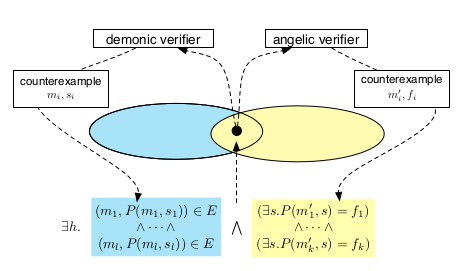
\includegraphics[scale=0.75]{solverarchitecture.png}
\end{center}
\caption{Sintetizer se sastoji od tri rešavača koji međusobno komuniciraju. Dva verifikatora generišu dve vrste kontraprimera i sintetizer generiše model koji zadovoljava ograničenja za sve kontraprimere.}
\label{fig:solver}
\end{figure}

\subsection{Upiti za analizu dvosmislenosti}
Nakon što je rešen problem sintetizovanja programa, potrebno je ispitati prostore mogućih modela. Ako je specifikacija nedovoljno precizna, teži se ka smanjenju dvosmislenosti proširivanjem specifikacije. Ako je specifikacija previše precizna, cilj je smanjiti specifikaciju bez stvaranja dvosmislenosti.\\\\

Skup objedinjenih ishoda programa, u oznaci $P[m]$, je skup ishoda programa $P$ nad mutacijom $m$ za sve rasporede $s$. Da bismo dobili ovakav skup, najpre, kreiramo ishod programa $P$ nad $m$ za inicijalni raspored $s$. Potom, uvećavamo skup uočenih ishoda $Obs$ traženjem rasporeda takvog, da program proizvodi do sada neviđeni ishod. Svaki korak algoritma doprinosi uvećanju skupa $Obs$ rešavanjem naredne formule:
\begin{equation}
\exists s. \wedge_{f \in Obs} P(m,s) \neq f
\end{equation}
Ako je ova formula zadovoljiva, dobili smo ishod koji možemo dodati u $Obs$, a potom pokušavamo ponovo da rešimo formulu sa dopunjenim skupom $Obs$. Ako je formula nezadovoljiva onda smo pronašli sve ishode programa $P$ za mutaciju $m$.

\section{Zaključak}
\label{sec:zakljucak}



\addcontentsline{toc}{section}{Literatura}
\appendix
\bibliography{seminarski} 
\bibliographystyle{plain}



\end{document}
